\section{Event categorization}
\label{sec:categorization}

In order to improve the sensitivity to the H boson production mechanisms,
the selected events are classified into mutually exclusive categories based on the features of the reconstructed objects associated with the $\PH\to4\ell$ candidates.
This categorization is primarily designed to separate $\ggH$, $\VBF$, $\VH$, and $\ttH$.
There is little sensitivity to $\bbH$ or $\tH$, even though these production modes are considered explicitly in the analysis.
The reconstructed event categories are further split (see Section~\ref{subsec:Reco_Categories}) in order to study deeper the structure within each production mechanisms.
This splitting is done matching the recommended binning of the framework of Simplified Template Cross Sections (STXS)~\cite{Bendavid:2018nar,YR4,Berger:2019wnu} that is described in Section~\ref{subsec:STXS_Categories}.

\subsection{STXS Production Bins}
\label{subsec:STXS_Categories}

The STXS were developed to provide more fine-grained measurements for individual H boson production modes in various kinematic regions and to reduce the theoretical uncertainties that are directly folded into the measurements.
The measured exclusive regions of phase space are referred to as production bins.
All production bins are defined using truth information in the MC simulation for H bosons with rapidity $|y_H|~<~2.5$, truth jets are defined as anti-\kt jets with a distance parameter of 0.4 and a $\pt$ threshold of 30\GeV, no requirement is placed on the particle-level leptons.
To account for the evolving experimental sensitivity, two stages of production bins with different granularity are considered.

The stage 0 production bins correspond to the H boson production mechanisms: $\tt ggH$, $\tt qqH$, $\tt VH$, and $\tt ttH$.
The $\tt qqH$ is the electroweak production bin that includes the production the H boson in association with two quarks from either $\VBF$ or $\VH$ events with hadronic decays of the vector boson V.
The $\tt VH$ production bin includes $\VH$ events with leptonic decays of the vector boson V.
The small $\bbH$ and $\tH$ production processes are considered together with the $\tt ggH$ and $\tt ttH$ production bins, respectively.
We study as well a modified version of the stage 0 production bins, where instead of $\tt VH$ and $\tt qqH$ bins we define the $\tt WH$, $\tt ZH$, and $\tt VBF$ bins that are mapping the respective H boson production mechanisms without the splitting of the VH events in leptonic and hadronic decays.

The stage 1.2 production bins are more granular than stage 0.
Several stage 1.2 production bins are merged as the full set of bins cannot be measured separately in this analysis with the current data sample.
The merged stage 1.2 production bins are discussed in more detail below.
\\
The $\ggH$ production process is split into events with $\pt^{\PH}<200$\GeV and $\pt^{\PH}>200$\GeV.
The events with $\pt^{\PH}>200$\GeV are placed into one single production bin called {\tt ggH/pT>200}.
The events with $\pt^{\PH}<200$\GeV are split in events with zero, one, and two or more jets.
The events with zero or one jets are split into the following production bins according to the H boson \pt : {\tt ggH-0j/pT[0,10]}, {\tt ggH-0j/pT[10-200]}, {\tt ggH-1j/pT[0-60]}, {\tt ggH-1j/pT[60-120]}, and {\tt ggH-1j/pT[120-200]}.
The events with two or more jets are split according to the dijet invariant mass as follows.
The events with $m_{jj}<350$\GeV are split into three production bins according to the H boson \pt: {\tt ggH-2j/pT[0-60]}, {\tt ggH-2j/pT[60-120]}, and {\tt ggH-2j/pT[120-200]}.
The events with $m_{jj}>350$\GeV are all placed into one production bin {\tt ggH-2j/mJJ>350}, which merges four bins originally suggested in stage 1.2 of the framework of STXS.
Fig.~\ref{fig:stage1_ggH} shows the merged stage 1.2 production bins used in the analysis for the $\ggH$ production process.
%=======
\begin{figure}[!htb]
	\vspace*{0.3cm}
	\begin{center}
		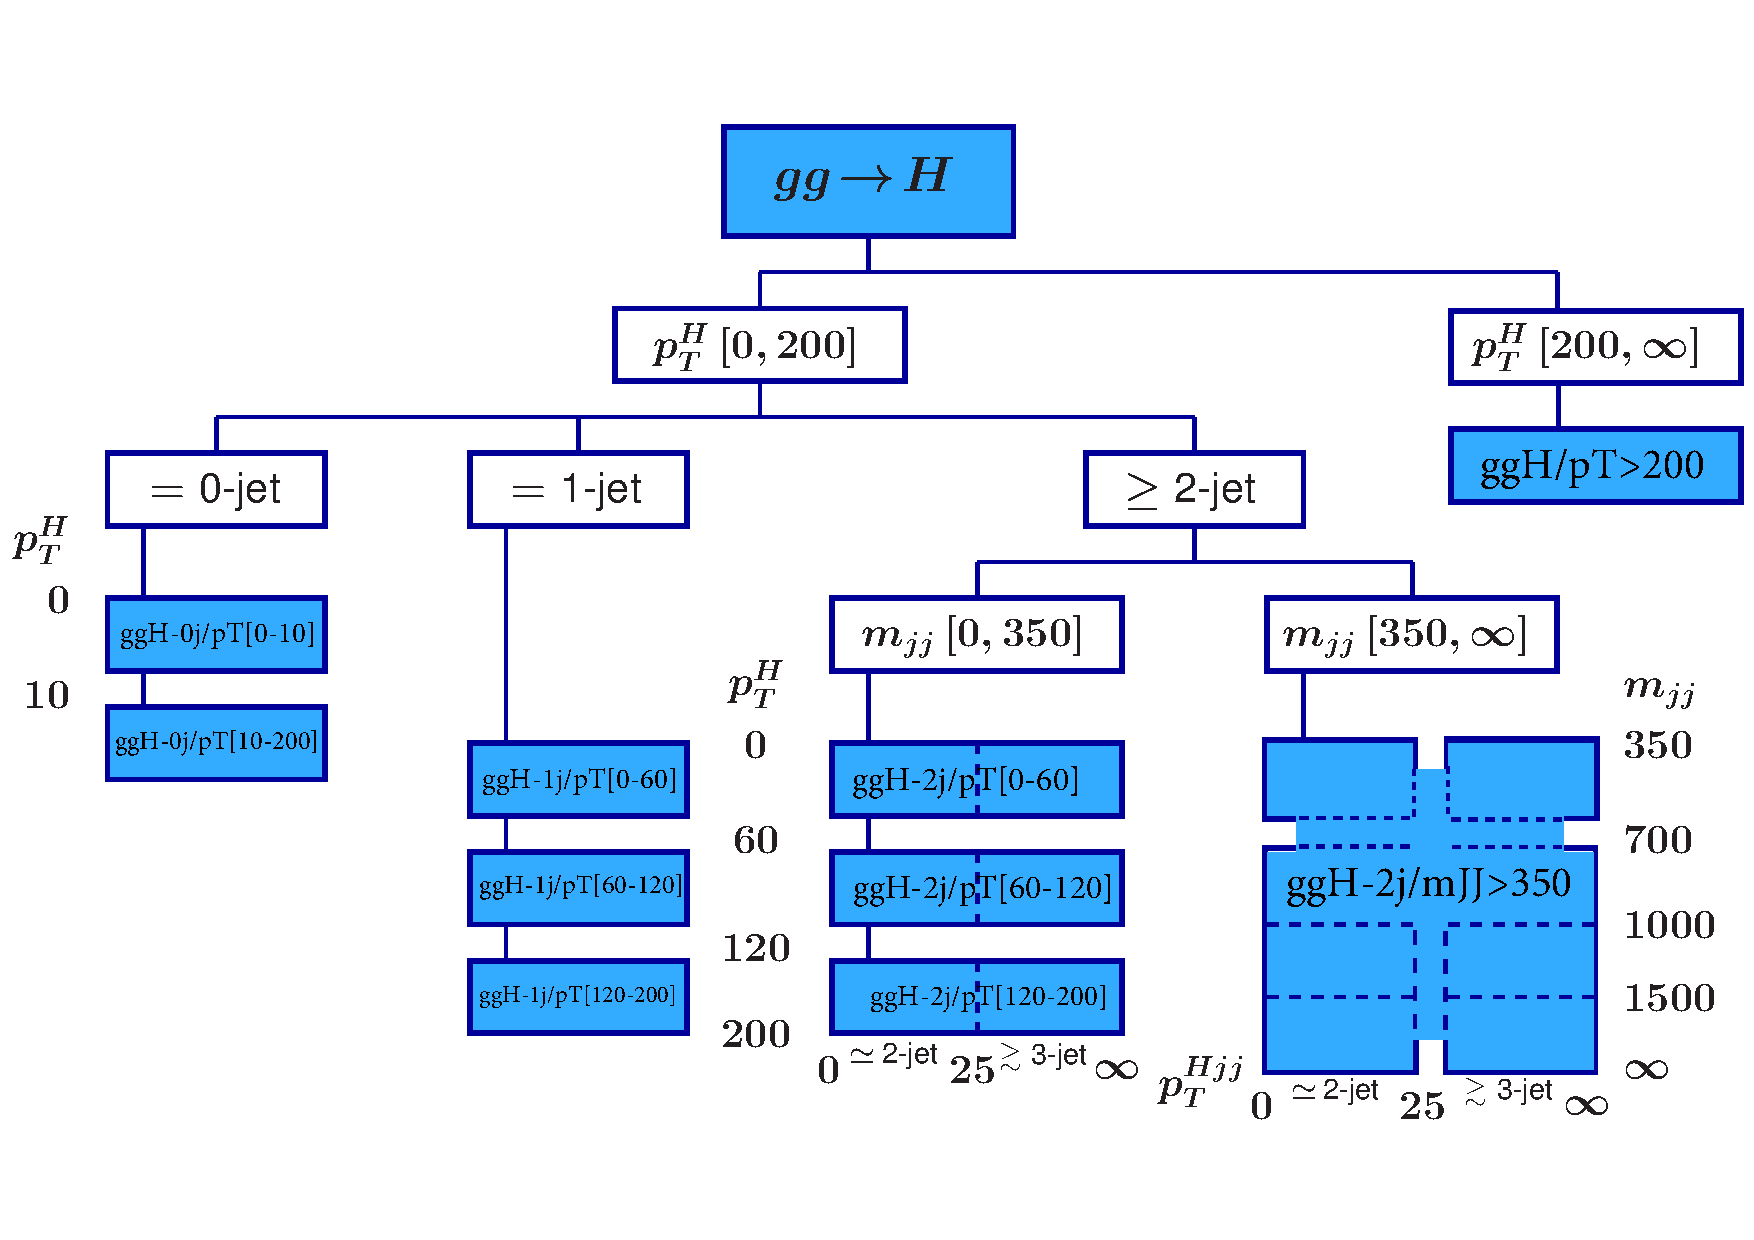
\includegraphics[width=0.8\textwidth]{Figures/stxs/simplifiedXS_ggF_11.pdf}
		\caption{Binning of the gluon fusion production process in the merged stage 1.2 of the framework of STXS~\cite{Berger:2019wnu} used in the analysis.
		\label{fig:stage1_ggH}}
	\end{center}
\end{figure}
%=======
\\
The electroweak $\tt qqH$ merged stage 1.2 production bins are sketched in Fig.~\ref{fig:stage1_VBF}.
The events with zero jet, one jet, or with two or more jets with $m_{jj}<60$\GeV or $120<m_{jj}<350$\GeV represent the production bins of secondary importance in the analysis and they are all merged into one bin called {\tt qqH-rest}.
The events with two or more jets and $60<m_{jj}<120$\GeV are placed in {\tt qqH-2j/mJJ[60-120]} bin.
The events with two or more jets and $m_{jj}>350$\GeV are split into events with $\pt^{\PH}<200$\GeV and $\pt^{\PH}>200$\GeV.
The events with $\pt^{\PH}>200$\GeV are placed into one single production bin called {\tt qqH-2j/pT>200}.
The events with $\pt^{\PH}<200$\GeV if $\pt^{\PH jj}<25$\GeV are split into two production bins {\tt qqH-2j/mJJ[350,700]} and {\tt qqH-2j/mJJ>700} and otherwise if $\pt^{\PH jj}>25$\GeV are merged in a single bin called {\tt qqH-3j/mJJ>350}.
%=======
\begin{figure}[!htb]
	\vspace*{0.3cm}
	\begin{center}
		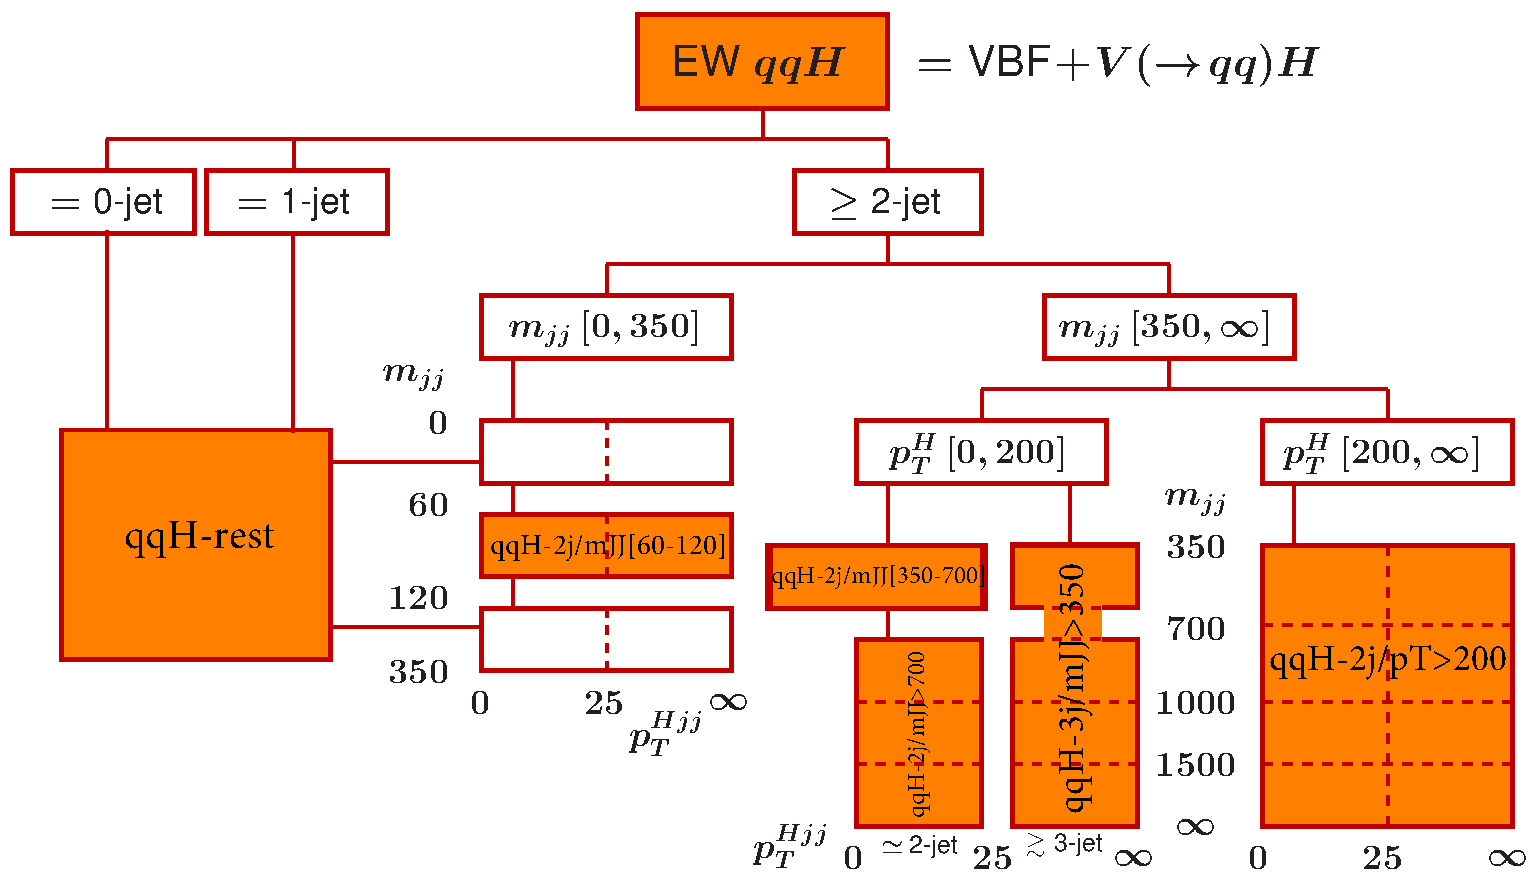
\includegraphics[width=0.8\textwidth]{Figures/stxs/simplifiedXS_VBF_11.pdf}
		\caption{Binning of the electroweak production process (combines VBF and VH with hadronic V decay) in the merged stage 1.2 of the framework of STXS~\cite{Berger:2019wnu} used in the analysis.
		\label{fig:stage1_VBF}}
	\end{center}
\end{figure}
%=======
\\
The $\tt VH$ reduced stage 1.2 production bins are shown in Fig.~\ref{fig:stage1_VH}.
The three production processes $\WH$, $\ZH$, and $\cPq\cPq\to\ZH$ are combined together.
Several proposed production bins are merged together into just two bins according to the \pt of the
vector boson: {\tt VH-lep/pTV[0-150]} and {\tt VH-lep/pTV>150}.
%=======
\begin{figure}[!htb]
	\vspace*{0.3cm}
	\begin{center}
		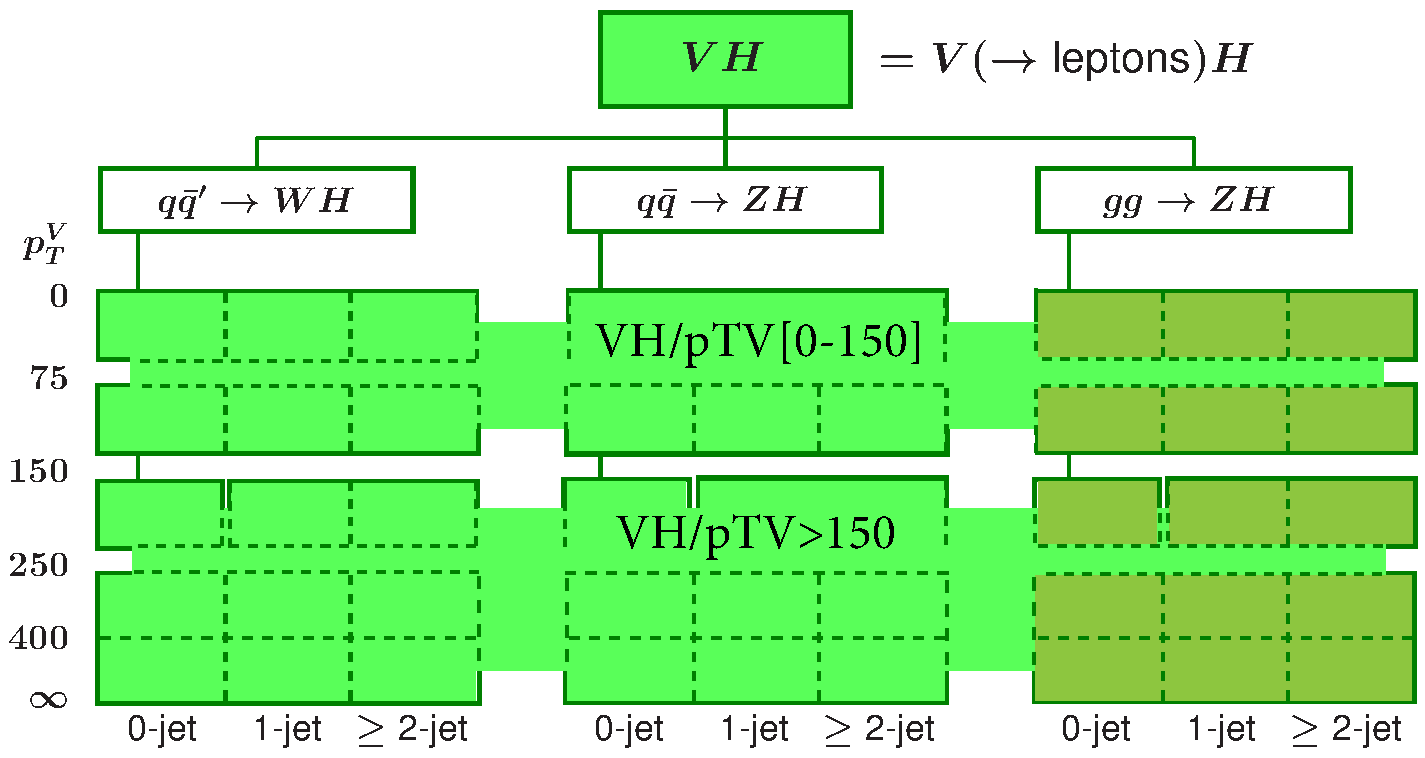
\includegraphics[width=0.8\textwidth]{Figures/stxs/simplifiedXS_VH_11.pdf}
		\caption{Binning of the VH production process with leptonic V decay (combining WH, ZH, and gluon fusion ZH production) in the merged stage 1.2 of the framework of STXS~\cite{Berger:2019wnu} used in the analysis.
		\label{fig:stage1_VH}}
	\end{center}
\end{figure}
%=======
\\
In stage 1.2 of the framework of STXS the {\tt ttH} stage 0 production bin is split in five different bins according to the \pt of the H boson.
Because of the very low expected yields all these bins are merged into a single stage 0 bin that includes the $\tH$ production process as well.
\\
Finally, in the stage 1.2 the small $\bbH$ production process is merged into the {\tt ggH-0j/pT[10-200]} production bin.


\subsection{Reconstructed Event Categories}
\label{subsec:Reco_Categories}


In order to be sensitive to different production bins, the $\cPZ\cPZ$ candidates that are passing the event selection described in Section~\ref{sec:objects} are classified into several dedicated reconstructed event categories.
The category definitions exploit the multiplicity of jets, b-tagged jets, and additional leptons not involved in the $\cPZ\cPZ$ candidate selection that satisfy identification, vertex compatibility, and isolation requirements.
Additional requirements on the kinematic discriminants described in Section~\ref{sec:observables}, the invariant mass of the two leading jets, and the transverse momentum of the ZZ candidate are also exploited.

The event categorisation is done in two steps.
In the first one, the $\cPZ\cPZ$ candidates are split in seven initial categories to target the main H boson production mechanisms corresponding to stage 0 production bins.
In the second one, more reconstructed event categories are determined to match the merged stage 1.2 production bins.

In the first categorisation step, the categories are defined, using the criteria applied in the following order (i.e. an event is considered for the subsequent category only if it does not satisfy the requirements of the previous category):
%
\begin{itemize}
\item[-] {$\VBF$-2jet-tagged} category requires exactly 4 leptons. In addition there must be either 2 or 3 jets
of which at most 1 is b-tagged, or at least 4 jets and no b-tagged jets. Finally, ${\cal D}_{\rm 2jet}>0.5$ is required.
\item[-] {$\VH$-hadronic-tagged} category requires exactly 4 leptons. In addition there must be 2 or 3 jets,
or at least 4 jets and no b-tagged jets. Finally, ${\cal D}_{\rm VH} > 0.5$ is required.
\item[-] {$\VH$-leptonic-tagged} category requires no more than 3 jets and no b-tagged jets in the event,
and exactly 1 additional lepton or 1 additional pair of opposite sign same flavor leptons. This category also includes events
with no jets and at least 1 additional lepton.
\item[-] {$\ttH$-hadronic-tagged} category requires at least 4 jets of which at least 1 is b-tagged and no additional leptons.
\item[-] {$\ttH$-leptonic-tagged} category requires at least 1 additional lepton in the event.
\item[-] {$\VBF$-1jet-tagged} category requires exactly 4 leptons, exactly 1 jet and ${\cal D}_{\rm 1jet}>0.7$.
\item[-] {Untagged} category consists of the remaining events.
\end{itemize}

In the second categorisation step, the {Untagged}, {$\VBF$-2jet-tagged}, {$\VH$-hadronic-tagged}, and {$\VH$-leptonic-tagged categories are further split.
A total number of 22 reconstructed event categories is defined, each of them is mainly matching a production bin (specified in brackets):

% \begin{itemize}
% \item {\bf Untagged category}:
% \end{itemize}
\begin{enumerate}
\itemsep0em

\item {\bf Untagged-0j-$\pt^{4\ell}[0,10]$} category requires the event in the Untagged category, no jets reconstructed, and $0<\pt^{4\ell}<10$\GeV ({\tt ggH-0j/pT[0-10]});

\item {\bf Untagged-0j-$\pt^{4\ell}[10,200]$} category requires the event in the Untagged category, no jets reconstructed, and $10<\pt^{4\ell}<200$\GeV ({\tt ggH-0j/pT[10-200]});

\item {\bf Untagged-1j-$\pt^{4\ell}[0,60]$} category requires the event in the Untagged category, one jet reconstructed, and $0<\pt^{4\ell}<60$\GeV ({\tt ggH-1j/pT[0-60]});

\item {\bf Untagged-1j-$\pt^{4\ell}[60,120]$} category requires the event in the Untagged category, one jet reconstructed, and  $60<\pt^{4\ell}<120$\GeV ({\tt ggH-1j/pT[60-120]});

\item {\bf Untagged-1j-$\pt^{4\ell}[120,200]$} category requires the event in the Untagged category, one jet reconstructed, and $120<\pt^{4\ell}<200$\GeV ({\tt ggH-1j/pT[120-200]});
\item {\bf Untagged-2j-$\pt^{4\ell}[0,60]$} category requires the event in the Untagged category, two jets reconstructed, $0<\pt^{4\ell}<60$\GeV, and $m_{jj}<350$\GeV ({\tt ggH-2j/pT[0-60]});

\item {\bf Untagged-2j-$\pt^{4\ell}[60,120]$} category requires the event in the Untagged category, two jets reconstructed, $60<\pt^{4\ell}<120$\GeV, and $m_{jj} <350$\GeV ({\tt ggH-2j/pT[60-120]});

\item {\bf Untagged-2j-$\pt^{4\ell}[120,200]$} category requires the event in the Untagged category, two jets reconstructed, $120<\pt^{4\ell}<200$\GeV, and $m_{jj} <350$\GeV ({\tt ggH-2j/pT[120-200]});

\item {\bf Untagged-$\pt^{4\ell}\gt200$} category requires the event in the Untagged category and $\pt^{4\ell}>200$ \GeV ({\tt ggH/pT>200});

\item {\bf Untagged-2j-$m_{jj}\gt350$} category requires the event in the Untagged category, two jets reconstructed, and $m_{jj} >$ 350\GeV ({\tt ggH-2j/mJJ>350});

\item {\bf $\VBF$-1jet-tagged} category ({\tt qqH-rest});

\item {\bf $\VBF$-2jet-tagged-$m_{jj}[350,700]$} category requires the event in the $\VBF$-2jet-tagged category, $\pt^{4\ell}<200$\GeV, $\pt^{4\ell jj}<25$\GeV, and $350<m_{jj}<700$\GeV ({\tt qqH-2j/mJJ[350-700]});

\item {\bf $\VBF$-2jet-tagged-$m_{jj}\gt700$} category requires the event in the $\VBF$-2jet-tagged category, $\pt^{4\ell}<200$\GeV, $\pt^{4\ell jj}<25$\GeV, and $m_{jj}>700$\GeV ({\tt qqH-2j/mJJ>700});

\item {\bf $\VBF$-3jet-tagged-$m_{jj}\gt350$} category requires the event in the $\VBF$-2jet-tagged category, $\pt^{4\ell}<200$\GeV, $\pt^{4\ell jj}>25$\GeV, and $m_{jj}>350$\GeV ({\tt qqH-3j/mJJ>350});

\item {\bf $\VBF$-2jet-tagged-$\pt^{4\ell}\gt200$} category requires the event in the $\VBF$-2jet-tagged category, $\pt^{4\ell}>200$ \GeV, and $m_{jj} >$ 350\GeV ({\tt qqH-2j/pT>200});

\item {\bf VBF-rest} category consists of the remaining events in the $\VBF$-2jet-tagged category ({\tt qqH-rest});

\item {\bf $\VH$-hadronic-tagged-$m_{jj}[60,120]$} category requires the event in the $\VH$-hadronic-tagged category and $60<m_{jj}<120$\GeV ({\tt qqH/mJJ[60-120]});

\item {\bf VH-rest} category consists of the remaining events in the $\VH$-hadronic-tagged category ({\tt qqH-rest});

\item {\bf $\VH$-leptonic-tagged-$\pt^{4\ell}[0,150]$} category requires the event in the $\VH$-leptonic-tagged category and $\pt^{4\ell} < 150$\GeV ({\tt VH-lep/pT[0-150]});

\item {\bf $\VH$-leptonic-tagged-$\pt^{4\ell}\gt150$} category requires the event in the $\VH$-leptonic-tagged category and $\pt^{4\ell} > 150$\GeV ({\tt VH-lep/pT>150});

\item {\bf $\ttH$-leptonic-tagged} category ({\tt ttH}).

\item {\bf $\ttH$-hadronic-tagged} category ({\tt ttH});

\end{enumerate}

Figure~\ref{fig:categ-purity-stage11} shows the signal relative purity of the merged stage 1.2 production bins in the 22 reconstructed event categories defined above.

%=======
\begin{figure}[!htb]
	\vspace*{0.3cm}
	\begin{center}
		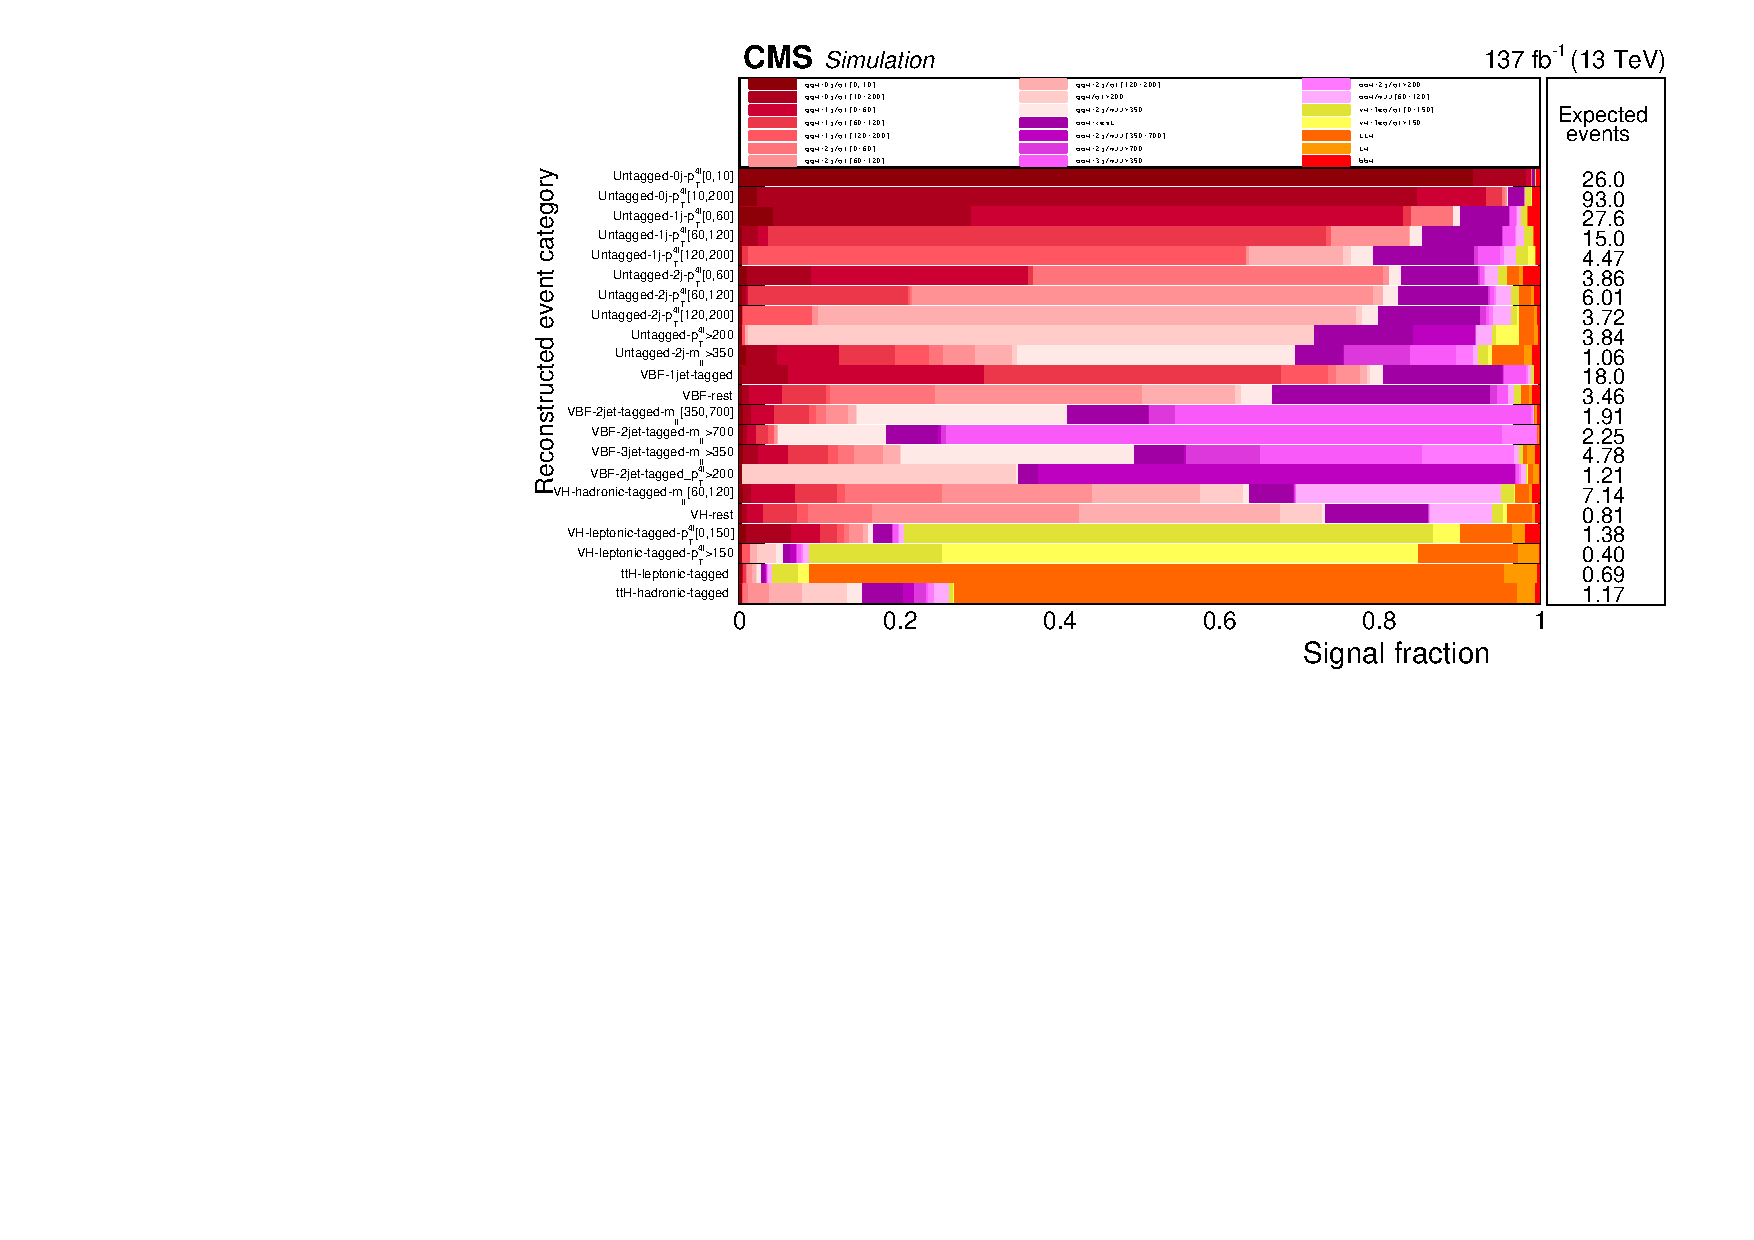
\includegraphics[width=1\textwidth]{Figures/stxs/STXS_Purity.pdf}
		\caption{Signal relative purity of the 22 reconstructed event categories in terms of merged stage 1.2 production bins in the $118<\mllll<130\GeV$ mass window.
			\label{fig:categ-purity-stage11}}
	\end{center}
\end{figure}
%=======